%!TEX program = xelatex
\documentclass[a4paper,UTF8]{article}
\usepackage{ctex}
\usepackage[margin=1.25in]{geometry}
\usepackage{color}
\usepackage{graphicx}
\usepackage{amssymb}
\usepackage{amsmath}
\usepackage{amsthm}
\usepackage{enumerate}
\usepackage{bm}
\usepackage{hyperref}
\usepackage{epsfig}
\usepackage{color}
\usepackage{mdframed}
\usepackage{lipsum}
\usepackage{graphicx}
\usepackage{float}
\newmdtheoremenv{thm-box}{Theorem}
\newmdtheoremenv{prop-box}{Proposition}
\newmdtheoremenv{def-box}{定义}

\usepackage{listings}
\usepackage{xcolor}
\lstset{
	numbers=left,
	numberstyle= \tiny,
	keywordstyle= \color{ blue!70},
	commentstyle= \color{red!50!green!50!blue!50},
	frame=shadowbox, % 阴影效果
	rulesepcolor= \color{ red!20!green!20!blue!20} ,
	escapeinside=``, % 英文分号中可写入中文
	xleftmargin=2em,xrightmargin=2em, aboveskip=1em,
	framexleftmargin=2em
}

\usepackage{booktabs}

\setlength{\evensidemargin}{.25in}
\setlength{\textwidth}{6in}
\setlength{\topmargin}{-0.5in}
\setlength{\topmargin}{-0.5in}
% \setlength{\textheight}{9.5in}
%%%%%%%%%%%%%%%%%%此处用于设置页眉页脚%%%%%%%%%%%%%%%%%%
\usepackage{fancyhdr}
\usepackage{lastpage}
\usepackage{layout}
\footskip = 12pt
\pagestyle{fancy}                    % 设置页眉
\lhead{2020年秋季}
\chead{神经网络}
% \rhead{第\thepage/\pageref{LastPage}页}
\rhead{作业一}
\cfoot{\thepage}
\renewcommand{\headrulewidth}{1pt}  			%页眉线宽,设为0可以去页眉线
\setlength{\skip\footins}{0.5cm}    			%脚注与正文的距离
\renewcommand{\footrulewidth}{0pt}  			%页脚线宽,设为0可以去页脚线

\makeatletter 									%设置双线页眉
\def\headrule{{\if@fancyplain\let\headrulewidth\plainheadrulewidth\fi%
\hrule\@height 1.0pt \@width\headwidth\vskip1pt	%上面线为1pt粗
\hrule\@height 0.5pt\@width\headwidth  			%下面0.5pt粗
\vskip-2\headrulewidth\vskip-1pt}      			%两条线的距离1pt
 \vspace{6mm}}     								%双线与下面正文之间的垂直间距
\makeatother

%%%%%%%%%%%%%%%%%%%%%%%%%%%%%%%%%%%%%%%%%%%%%%
\numberwithin{equation}{section}
%\usepackage[thmmarks, amsmath, thref]{ntheorem}
\newtheorem{theorem}{Theorem}
\newtheorem*{definition}{Definition}
\newtheorem*{solution}{Solution}
\newtheorem*{prove}{Proof}
\newcommand{\indep}{\rotatebox[origin=c]{90}{$\models$}}

\usepackage{multirow}

%--

%--
\begin{document}
\title{神经网络\\
作业四}
\author{181220076, 周韧哲, zhourz@smail.nju.edu.cn}
\maketitle

\section*{Problem 1}
设计双月数据,使其线性不可分,用单层感知器和BP神经网络分别进行分类,比较其结果。尝试分析BP网络隐藏神经元在非线性分类中所起的作用。
\begin{solution}.\\
如下图\ref{fig:1}中的左图为产生的双月数据,一共$2000$个点;中间图为$BP$神经网络的分类结果;右图为单层感知机的分类结果。我设计了一个拥有$3$层隐藏层的$\text{BP}$网络,其中隐藏层激活函数为$relu$,隐藏层神经元个数为$32$,输出层激活函数为$sigmoid$,学习率设置为$0.0003$,迭代$200$轮后分类正确率为$100\%$。单层感知机的激活函数为sigmoid函数,迭代$200$轮后分类正确率为$91.25\%$。命令行输入$\textbf{python double\_moon.py ---hidden\_layer\_num 3}$和$\textbf{python double\_moon.py ---hidden\_layer\_num 0}$运行可复现结果。\\
可以看出,单层感知机无法处理线性不可分数据,而多层BP网络可以很好地分类线性不可分数据。隐藏神经元或者说隐藏层的权重矩阵,能够把数据特征抽象到另一个维度空间,从而对输入特征进行了多层次的抽象:矩阵和向量相乘,本质上就是对向量的坐标空间进行一个变换。因此,隐藏层的权重矩阵的作用就是使得数据的原始坐标空间从线性不可分,转换成了线性可分。
\end{solution}
\begin{figure}[!htb]
	\centering
	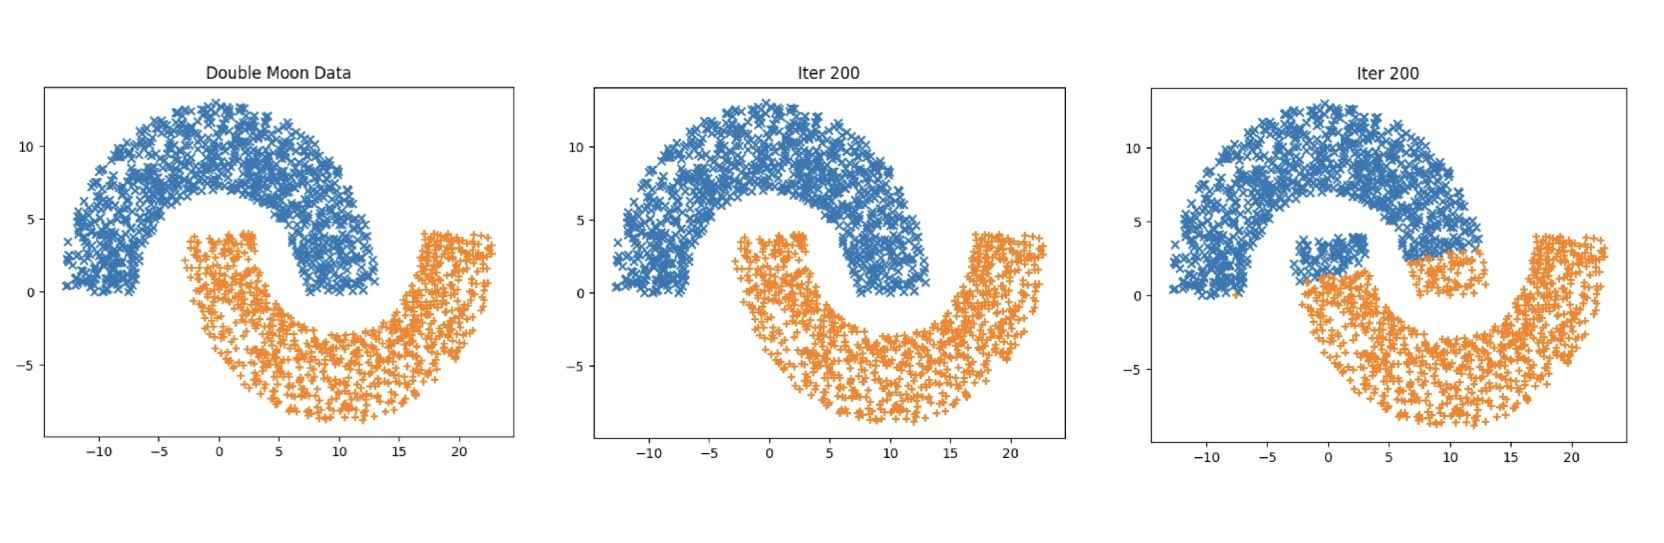
\includegraphics[width=\textwidth]{pic/1.png}
	\label{fig:1}
	\caption{P1}
\end{figure}
\section*{Problem 2}
从网上下载optdigits数据库,这是一个10类手写数字库。建立一个BP网络用于这个10类手写数字的分类,使用一层隐藏层。用training集对该网络进行训练,用test集测试。
\begin{enumerate}[(1)]
	\item 比较不同的隐藏层神经元个数对结果有什么影响。
	\item 思考如何进一步提高识别率。
\end{enumerate}

\begin{solution}.
	\begin{enumerate}[(1)]
		\item 命令行输入$\textbf{python optdigits.py ---hidden\_dim 128}$运行可以训练网络并在测试集上测试。使用一层隐藏层,固定迭代$100$轮,当隐藏神经元个数为$16,32,64,128,256$时,在测试集上的准确率分别为$0.9137,0.9399,0.9572,0.9594,0.9599$。直观来看,隐藏层神经元个数越多,分类准确率越高,因为神经元个数越多,表示能力越强。
		\item 通过增加隐藏层数量、提高训练轮数、调节学习率,可以进一步提高识别率。当迭代$120$轮,隐藏层神经元个数为$128$,隐藏层数量为$2$,学习率为$0.002$时,在测试集上的准确率达到了$0.9627$。通过调参得到较好的学习率、迭代次数、不同激活函数,或者通过归一化输入数据也可以提高网络模型的效果。
	\end{enumerate}
\end{solution}
\section*{Problem3}
训练一个1-5-1的神经网络来逼近函数sin(x):
\begin{enumerate}[(1)]
	\item 由sin函数产生100个输入-输出对,训练该神经网络使其能根据x预测sin(x),报告其精度(误差)。
	\item 报告输入-隐藏层权值及隐藏-输出层权值。
	\item 报告作为x的函数的隐藏神经元输出y,报告输出神经元的输出z,找到每一个隐藏神经元输出函数的分界点,讨论参与产生输出的隐藏神经元。
\end{enumerate}
\begin{solution}.
\begin{enumerate}[(1)]
	\item 命令行输入$\textbf{python sinx.py}$运行可得到结果,最终迭代500轮,均方误差约为$0.04216$。
	\item 输入-隐藏层权值为:\begin{align*}
		w_0&=[0.91403577,-0.63624996,-0.02249133,1.08801627,0.18224804]\\
		b_0&=[0.89582971,-0.80988285,-0.09036633,-1.35959951,0.17857199]
	\end{align*}
    隐藏-输出层权值为:\begin{align*}
    	w_1&=[1.20082916,0.89272928,-0.1035579,-1.65504323,0.23501796]\\
    	b_1&=[-1.12173529]
    \end{align*}
    \item 隐藏神经元的激活函数为relu,输出y见文件$\textbf{data/layer0\_output.txt}$。输出神经元的激活函数为tanh,输出z见文件$\textbf{data/layer1\_output.txt}$。观察输出易知参与产生输出的包括了所有隐藏神经元。
\end{enumerate}
\end{solution}
\end{document}